\section{Robust Geometric Programming} \label{RGP}

This section presents a brief review of the approximation of an RGP as a
tractable optimization problem as discussed in~\cite{Saab2018}.
The robust counterpart of an uncertain geometric program is:

\begin{equation}
\begin{aligned}
& \min &&f_0\left(\vec{x}\right)\\
& \text{subject to} &&\max_{\vec{\zeta} \in \mathcal{Z}} \left\{\textstyle{\sum}_{k=1}^{K_i}e^{\vec{a_{ik}}\left(\zeta\right)\vec{x} + b_{ik}\left(\zeta\right)}\right\} &&\leq 1 &&\forall i \in 1,...,m\\
\end{aligned}
\label{GP_counterparts_finite}
\end{equation}

which is Co-NP hard in its natural posynomial form \cite{RGPcoNP}. We will present three approximate formulations of a \gls{rgp}.

\subsection{Simple Conservative Formulation}
One way to approach the intractability in \eqref{GP_counterparts_finite} is to replace each constraint by a tractable approximation.
Replacing the max-of-sum in \eqref{GP_counterparts_finite} by the sum-of-max will lead to the following formulation

\begin{equation}
\begin{aligned}
& \min &&f_0\left(\vec{x}\right)\\
& \text{subject to} &&\textstyle{\sum}_{k=1}^{K_i} {\displaystyle \max_{\vec{\zeta} \in \mathcal{Z}}} \left\{e^{\vec{a_{ik}}\left(\zeta\right)\vec{x} + b_{ik}\left(\zeta\right)}\right\} &&\leq 1 &&\forall i \in 1,...,m
\end{aligned}
\label{GP_safe_conservative}
\end{equation}
Maximizing a monomial term is equivalent to maximizing an affine function, therefore \eqref{GP_safe_conservative} is tractable.

\subsection{Equivalent Intermediate Formulation}

This formulation is equivalent to the formulation in \eqref{GP_counterparts_finite}, but with smaller, easier to handle posynomial constraints.
By the properties of inequalities, the posynomial $P$ in posynomial inequality $ M \geq  P$ can be
divided into an equivalent set of smaller posynomials based on the dependence between its monomial terms.
Figure~\ref{fig:partitioning} shows how a constraint can be represented as an equivalent set of smaller posynomial constraints.

\begin{figure}
    \begin{center}
        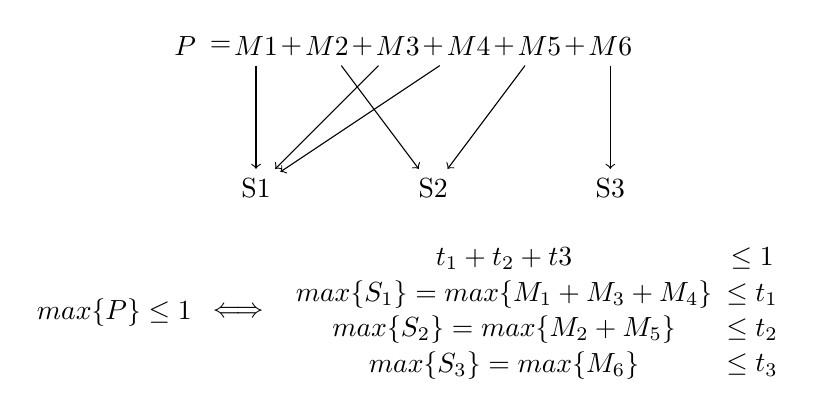
\begin{tikzpicture}[auto,scale = 0.9]
            \begin{scope}[node distance=0.5cm]
                \node[name=P] at (0,0) (P) {$P$};
                \node[name=equals] at (0.5,0) (equals) {$=$};
                \node[name=M1] at (1,0) (M1) {$M1$};
                \node[name=M2] at (2,0) (M2) {$M2$};
                \node[name=M3] at (3,0) (M3) {$M3$};
                \node[name=M4] at (4,0) (M4) {$M4$};
                \node[name=M5] at (5,0) (M5) {$M5$};
                \node[name=M6] at (6,0) (M6) {$M6$};
                \node[name=p1] at (1.5,0) (p1) {$+$};
                \node[name=p2] at (2.5,0) (p2) {$+$};
                \node[name=p3] at (3.5,0) (p3) {$+$};
                \node[name=p4] at (4.5,0) (p4) {$+$};
                \node[name=p5] at (5.5,0) (p5) {$+$};
                \node[name=S1] at (1,-2) (S1) {S1};
                \node[name=S2] at (3.5,-2) (S2) {S2};
                \node[name=S3] at (6,-2) (S3) {S3};
                \draw[->] (M1) -- (S1);
                \draw[->] (M3) -- (S1);
                \draw[->] (M4) -- (S1);
                \draw[->] (M2) -- (S2);
                \draw[->] (M5) -- (S2);
                \draw[->] (M6) -- (S3);
                \node[name=t1, align=left] at (8, -3) (t1) {$\leq 1$};
                \node[name=t2, align=left] at (8, -3.5) (t1) {$\leq t_1$};
                \node[name=t3, align=left] at (8, -4) (t1) {$\leq t_2$};
                \node[name=t4, align=left] at (8, -4.5) (t1) {$\leq t_3$};
                \node[name=arrow] at (0.75,-3.75) (arrow) {$\Longleftrightarrow$};
                \node[name=orig] at (-1,-3.75) (orig) {$max\{P\} \leq 1$};
                \node[name=c1, align=left] at (4.5,-3) (c1) {$t_1 + t_2 + t3$};
                \node[name=c2, align=left] at (4.5,-3.5) (c2) {$max\{S_1\} = max\{M_1 + M_3 + M_4\}$};
                \node[name=c3, align=left] at (4.5,-4) (c3) {$max\{S_2\} = max\{M_2 + M_5\}$};
                \node[name=c4, align=left] at (4.5,-4.5) (c4) {$max\{S_3\} = max\{M_6\}$};

            \end{scope}
        \end{tikzpicture}
        \caption{Partitioning of a large posynomial into smaller posynomials requires the addition of auxiliary variables. $S_i$
        are posynomials with independent sets of variables.}
        \label{fig:partitioning}
    \end{center}
\end{figure}

The posynomial constraints are categorized into three sets: large posynomials, two-term posynomials and monomials,
represented by $S1$, $S2$ and $S3$ respectively.
Monomials are tractable, and two-term posynomials can be well approximated using piecewise-linear
functions~\cite{hsiung_kim_boyd_2007}.
We implement the following two tractable approximations for large posynomials.

\subsubsection{Linearized Perturbations Formulation}
If the exponents are known and certain, then large posynomial constraints can be approximated as signomial constraints.
The exponential perturbations in each posynomial are linearized using a modified least squares method, and then the
posynomial is robustified using techniques from robust linear programming. The resulting set of constraints is \gls{sp} compatible,
therefore, a robust geometric program can be approximated as a signomial program.

\subsubsection{Best Pairs Formulation}
If the exponents are also uncertain, then large posynomials can't be approximated as an \gls{sp}, and further simplification is needed.
This formulation aims to maximize each pair of monomials in each posynomial,
while finding the best combination of monomials that gives the least conservative solution.
\cite{Saab2018} provides a descent algorithm to find locally optimal combinations of the monomials,
and shows how the uncertain geometric program can be approximated as a geometric program for polyhedral uncertainty,
and a conic optimization problem for elliptical uncertainty with uncertain exponents.
For a detailed description of the above formulations refer to \cite{Saab2018}.
An algorithm for solving an \gls{rsp} based on the above formulations is provided in the next section.
